\documentclass[letterpaper,12pt]{article}
\usepackage[utf8]{inputenc}
\usepackage{fullpage}
\usepackage{courier}
\usepackage[margin=0.75in]{geometry}
\usepackage{listings}
\usepackage{color}
\usepackage{graphicx}
\usepackage[width=4in]{caption}
\usepackage{hyphenat}
\usepackage{multicol}

% Format a sectionless paragraph
\newcommand*\unparagraph{
	\par
	\nopagebreak
	\vskip3.25ex plus1ex minus.2ex
	\noindent
}

% define extra colors
\definecolor{dkgreen}{rgb}{0,0.6,0}
\definecolor{purple}{RGB}{159,0,197}

% define the code listing format
\lstset{
	language=C++,
	basicstyle=\ttfamily,
	backgroundcolor=\color{white},
	showspaces=false,
	showstringspaces=false,
	%frame=single,
	tabsize=3,
	keywordstyle=\color{purple},
	commentstyle=\color{dkgreen},
	stringstyle=\color{blue},
	escapeinside={\%*}{*)},
	morekeywords={cout,cin,endl}
}

% efine the title/header
\title{\Large CS 1428\\Lab 6 Section 06} 
\author{Jared Wallace}
\date{}

\begin{document}

\maketitle

\section*{Topic}
Today we learn about \textbf{for} loops. A \textbf{for} loop allows us to repeat a certain segment of 
code when we know ahead of time exactly how many repetitions we want to occur.  There
are three parts to a \textbf{for} loop. The declaration/initialization of the index variable, the limit, and 
the step.

% code example here
\unparagraph{}
\begin{lstlisting}[basicstyle=\footnotesize\ttfamily]
// example of a for loop
cout << "I'm going to count to 10!" << endl;

for (int i = 1; i <= 10; ++i)
{
   cout << i << endl;
}


"""""""""""""""""""""""""""""""""""""""""""""""""""""""""""""""""""""""""
Output:

I'm going to count to 10!
1
2
3
4
5
6
7
8
9
10
\end{lstlisting}

\newpage

\section*{Questions}
\begin{enumerate}
	\item Fill in the blanks so that the following code fragment prints out \lstinline$0.2,0.4,0.6,0.8,1$:

\begin{lstlisting}[frame=none]
for (int i = 2; i <= 10; i += 2)
{
   float value = ____________;
   cout << ________ << ",";
}
cout << endl;
\end{lstlisting}

	\item What would the following code print out to the screen?

\begin{lstlisting}[frame=none]
for (int i = 0; i < 5; ++i)
{
   for(int j = 0; j < 10; ++j)
   {
      cout << "*";
   }
   cout << endl;
}
\end{lstlisting}

		\begin{multicols}{2}
		\begin{enumerate}
			\item

\begin{lstlisting}[frame=none]
**********
**********
**********
**********
**********
\end{lstlisting}

			\item 

\begin{lstlisting}[frame=none]
**********
**********
**********
**********
**********
**********
**********
**********
**********
**********
\end{lstlisting}

			\item 

\begin{lstlisting}[frame=none]
*****
*****
*****
*****
*****
*****
*****
*****
*****
*****
\end{lstlisting}

			\item 

\begin{lstlisting}[frame=none]
*
*
*
*
*
\end{lstlisting}


		\end{enumerate}
		\end{multicols}

		\item What is the output of the following code fragment?

\begin{lstlisting}[frame=none]
for (int count = 0; count <= 9; ++count)
{
   cout << count << " ";
}
cout << endl;
\end{lstlisting}

			\begin{multicols}{2}
			\begin{enumerate}
				\item 0 1 2 3 4 5 6 7 8
				\item 0 1 2 3 4 5 6 7 8 9
				\item 0 1 2 3 4 5 6 7
				\item 1 2 3 4 5 6 7 8 9
			\end{enumerate}
			\end{multicols}

\end{enumerate}



\section*{Programming Exercise}
For this program you will need to use nested for loops to accomplish to goal.  You will
prompt the user for a number between 1 and 25.  If the number entered is not acceptable
then the program should print out a message informing the user and then exit.  Once a 
valid input is accepted you will print out a triangle of numbers.  For example, if the
number entered was 9 then the triangle would look like this:

\begin{lstlisting}[frame=none]
987654321
87654321
7654321
654321
54321
4321
321
21
1
\end{lstlisting}

When tackling the triangle think about which for loop is responsible for the lines and which one 
is responsible for the characters in a single line $($in what order are they printed to the screen$)$

\vspace{15mm}

% Don't forget the submission instructions!
\unparagraph{} \textbf{When you are done submit your source code via the online homework submission site.
Then staple a printout of the source to the back of this handout $($Don't forget to answer the questions above!$)$
and turn the packet in, face down, on my desk.}

\vspace{15mm}

% Comic at the bottom
\begin{figure}[ht!]
	\centering
	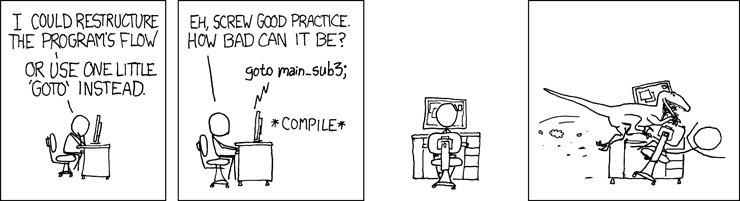
\includegraphics[width=6in]{goto.png}
	\caption*{Neal Stephenson thinks it's cute to name his labels \lq dengo\rq}
\end{figure}

\end{document}
